\section{Hardware Design}
The hardware architecture of the Smart Plant Watering System was designed to be modular and resilient. This section describes the choice of components, the pin mapping, and the electronics analysis.

\subsection{Key Components}
Each hardware element has been selected for its reliability and compatibility with the 5V logic of the PIC16F1789.

\subsubsection{Microcontroller (PIC16F1789)}
The central logic unit of the system. This 8-bit MCU handles all sensor acquisitions, timing through interruptions, and the I2C communication protocol for the display.

\begin{figure}[H]
    \centering
    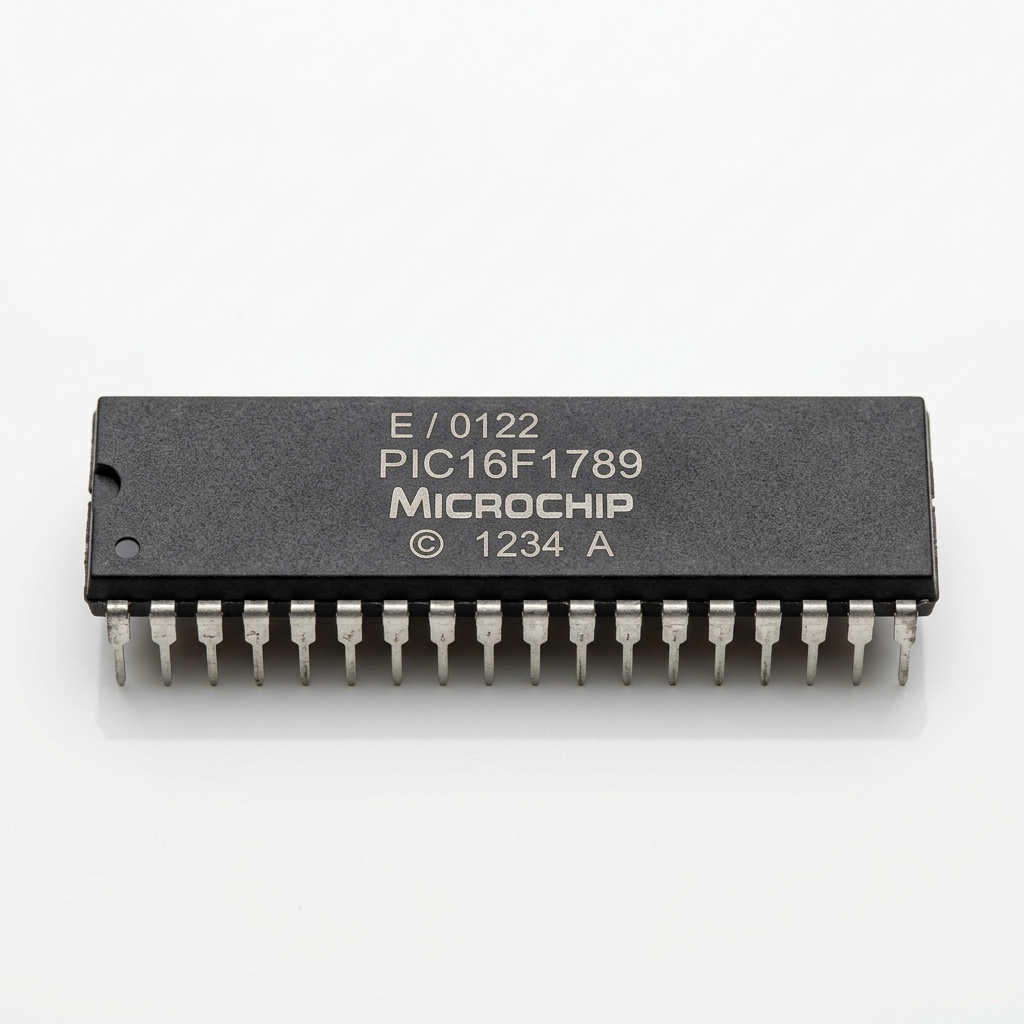
\includegraphics[width=0.4\linewidth]{images/mcu.png}
    \caption{PIC16F1789 Microcontroller in 40-pin DIP package.}
\end{figure}

\subsubsection{Capacitive Soil Moisture Sensor}
The SEN0308 sensor measures soil moisture by detecting changes in capacitance. Unlike resistive sensors, its electrodes are not exposed to the soil, preventing corrosion and ensuring long-term measurement stability.

\begin{figure}[H]
    \centering
    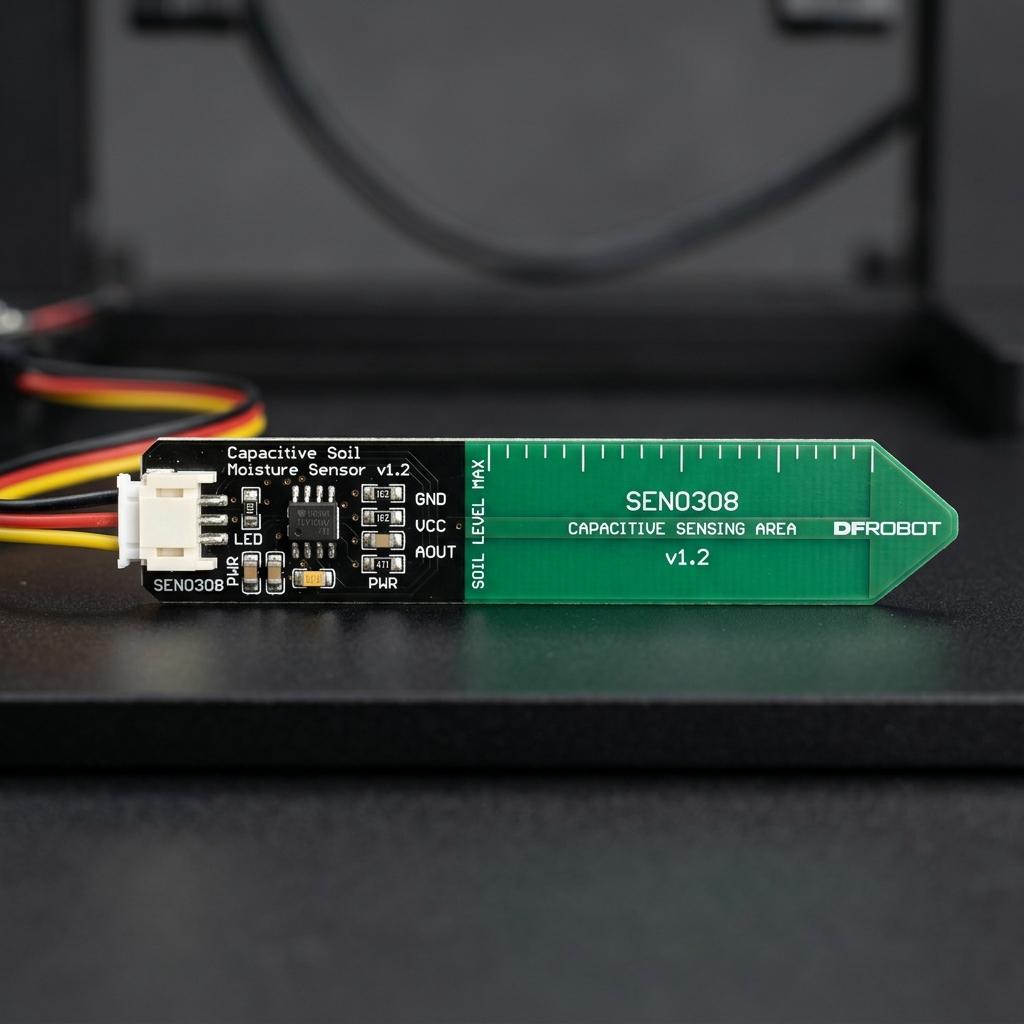
\includegraphics[width=0.4\linewidth]{images/sensor.png}
    \caption{Capacitive soil moisture sensor (SEN0308).}
\end{figure}

\subsubsection{Submersible Pump (9V DC)}
A compact FIT0563 pump used to deliver water from the reservoir to the plant. It is powered by a dedicated 9V source to avoid electrical noise on the logic rails.

\begin{figure}[H]
    \centering
    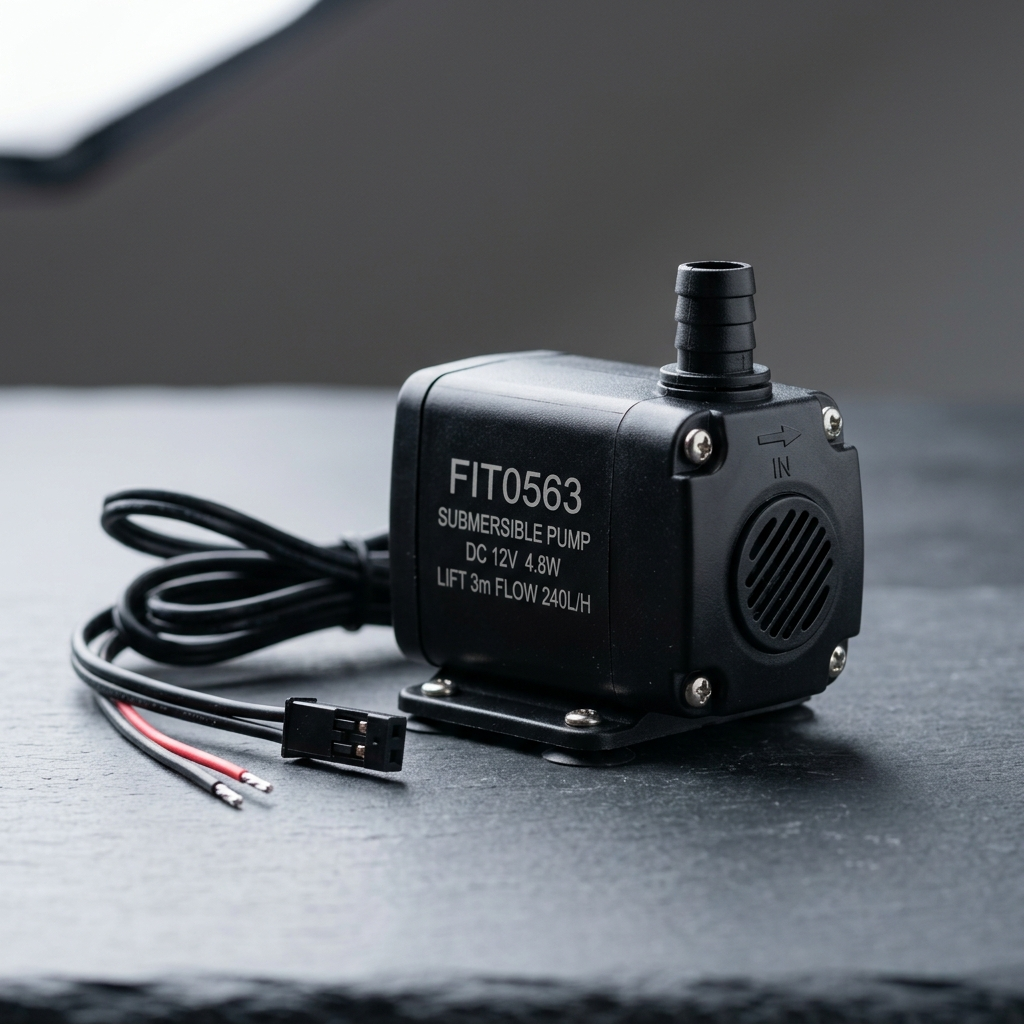
\includegraphics[width=0.35\linewidth]{images/pump.png}
    \caption{9V DC submersible water pump.}
\end{figure}

\subsubsection{LCD I2C Display (16x2)}
An alphanumeric display that provides the user with real-time data. The I2C interface allows for full control of the 16x2 screen using only two pins (SDA/SCL).

\begin{figure}[H]
    \centering
    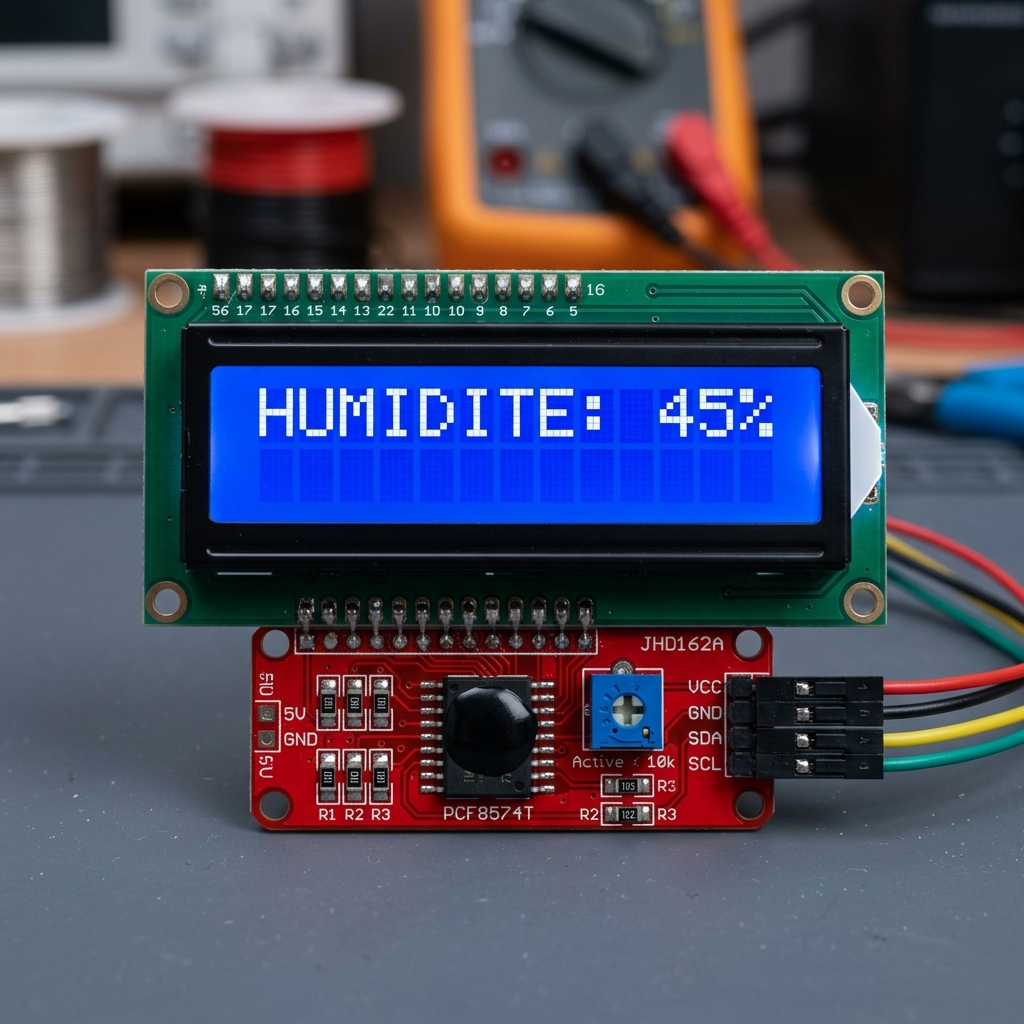
\includegraphics[width=0.45\linewidth]{images/lcd.png}
    \caption{16x2 Character LCD with I2C backpack.}
\end{figure}

\subsubsection{5V Relay Module}
This module acts as an interface between the low-power microcontroller signal and the high-power pump circuit, providing essential galvanic isolation.

\begin{figure}[H]
    \centering
    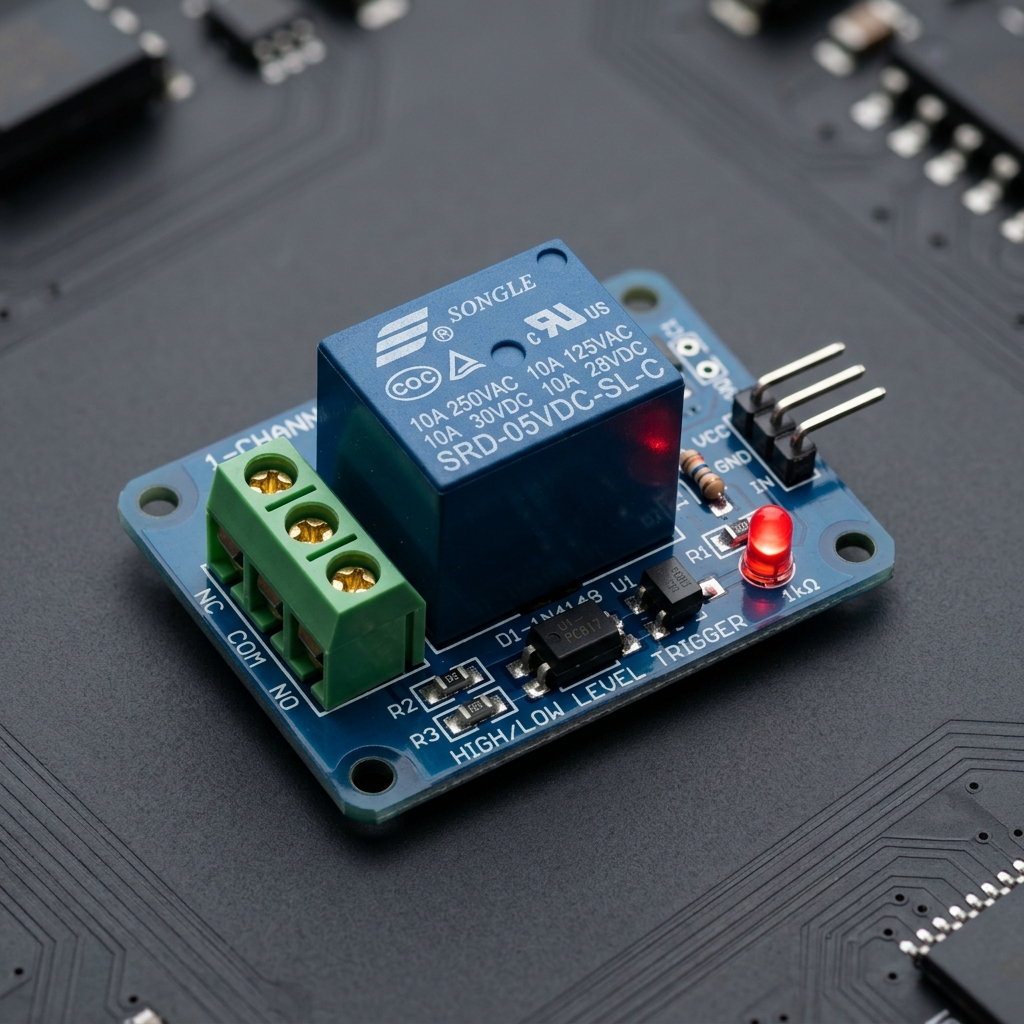
\includegraphics[width=0.4\linewidth]{images/relay.png}
    \caption{Single-channel 5V relay module.}
\end{figure}

\subsection{Development and Power Tools}
The following tools were essential for the development, programming, and power regulation of the system.

\subsubsection{MPLAB Snap Programmer}
The primary tool for In-Circuit Serial Programming (ICSP). It connects the PC to the PIC16F1789 for firmware uploading and real-time debugging.

\begin{figure}[H]
    \centering
    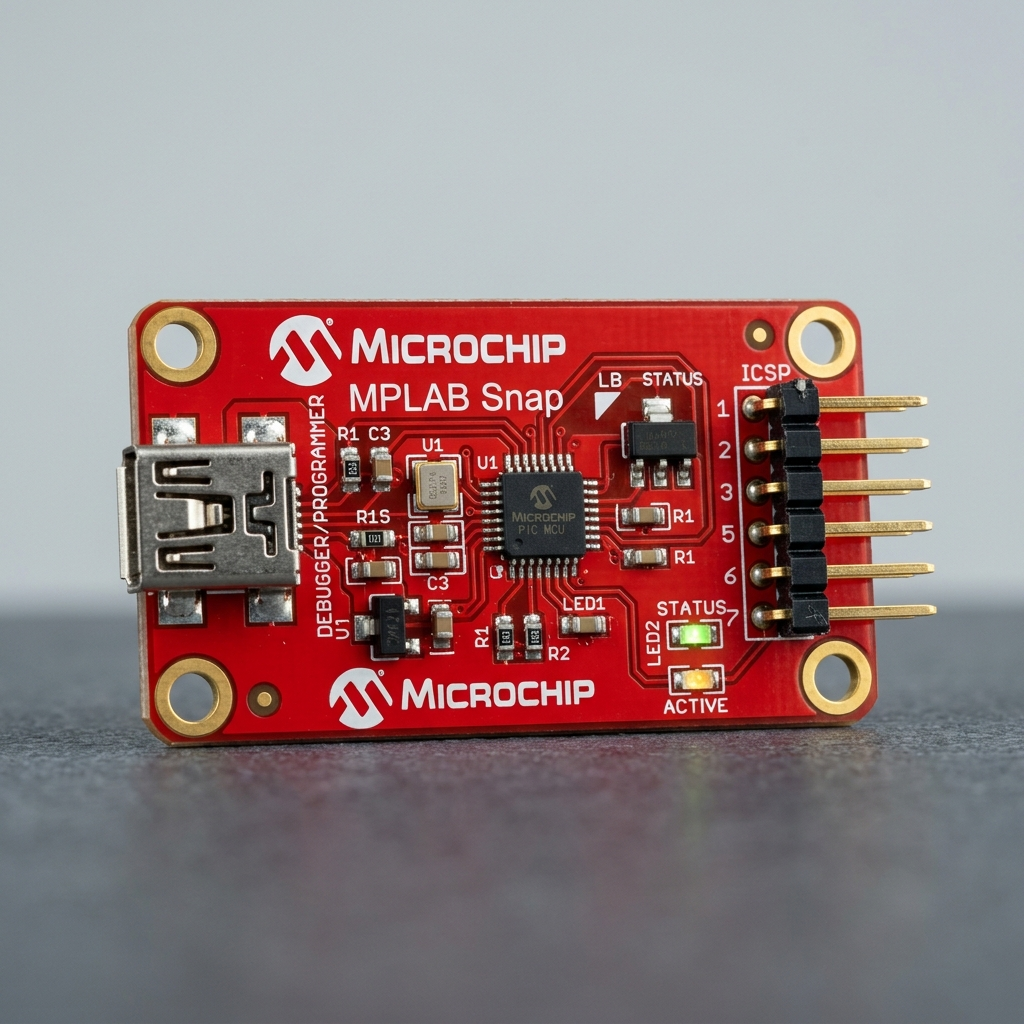
\includegraphics[width=0.4\linewidth]{images/programmer.png}
    \caption{MPLAB Snap debugger and programmer.}
\end{figure}

\subsubsection{MB102 Power Module}
A breadboard-mounted regulator that converts external DC power into stable 5V and 3.3V rails, ensuring a clean power supply for the microcontroller.

\begin{figure}[H]
    \centering
    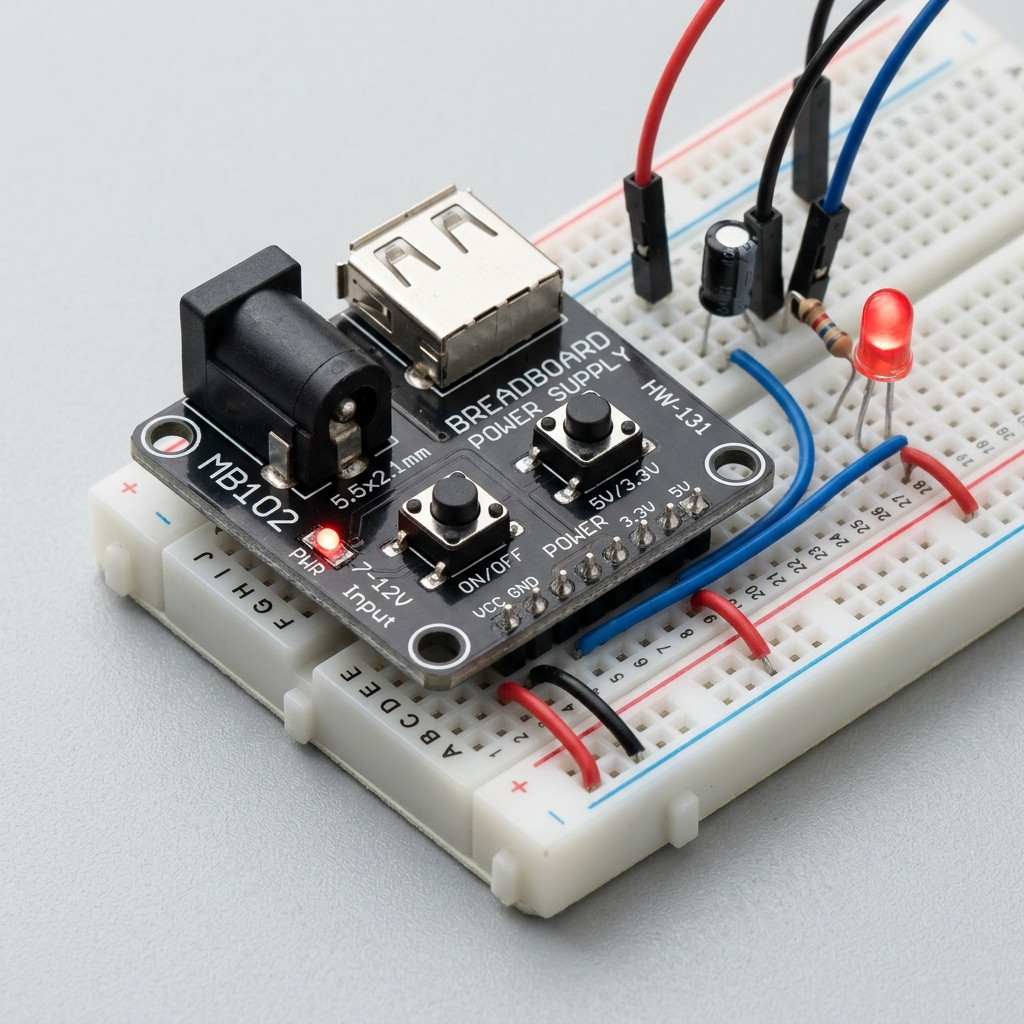
\includegraphics[width=0.45\linewidth]{images/power.png}
    \caption{MB102 breadboard power supply module.}
\end{figure}

\subsection{Pin Mapping and Connectivity}
The following table summarizes the physical connections between the PIC16F1789 and the peripheral components.

\begin{table}[H]
\centering
\begin{tabular}{|l|l|l|l|}
\hline
\textbf{Pin Name} & \textbf{Pin \#} & \textbf{Function} & \textbf{Description} \\ \hline
RA1 & 3 & Output (Digital) & Sensor Power Control (HYGRO\_POWER) \\ \hline
RA2 & 4 & Input (Analog) & Soil Moisture Signal (ANA2) \\ \hline
RB0 & 33 & Input (Pull-up) & System ON/OFF Switch \\ \hline
RB1 & 34 & Input (Pull-up) & Manual Pump Override Button \\ \hline
RB2 & 35 & Input (Pull-up) & Info/Slideshow Toggle Button \\ \hline
RC3 & 18 & Output (Digital) & I2C Serial Clock (SCL) \\ \hline
RC4 & 23 & Output/Input & I2C Serial Data (SDA) \\ \hline
RD0 & 19 & Output (Digital) & Pump Relay Control (Active Low) \\ \hline
RD1 & 20 & Output (Digital) & Green Status LED \\ \hline
RD2 & 21 & Output (Digital) & Red Standby LED \\ \hline
\end{tabular}
\caption{Pin assignment for the PIC16F1789 controller.}
\end{table}

\subsection{Electronics Analysis}
\subsubsection{Sensor Power Management}
To prevent electrolysis and unnecessary power consumption, the moisture sensor is not powered continuously. The PIC16F1789 controls the sensor's VCC through the \texttt{HYGRO\_POWER\_PIN} (RA1). It is only powered 50ms before an ADC conversion and shut down immediately after.

\subsubsection{Input Protection and Pull-ups}
All user buttons (RB0-RB2) utilize the microcontroller's internal Weak Pull-Up (WPU) resistors. This simplifies the PCB design by eliminating external resistors while ensuring a stable logic "1" state when the buttons are not pressed.

\subsubsection{Pump Power and Relay Control}
The submersible pump requires a 9V DC supply and a high starting current that the PIC16F1789 cannot provide directly. To solve this, a dual-supply architecture was implemented:
\begin{itemize}
    \item \textbf{Logic Power:} The microcontroller and sensor are powered by a regulated 5V supply from the breadboard power module.
    \item \textbf{Power Load:} The pump is connected to an external 9V battery (or DC adapter).
\end{itemize}
The 5V relay module acts as an electromagnetic switch. When the \texttt{RELAY\_PUMP\_PIN} (RD0) is driven low, the relay's internal coil is energized, closing the 9V circuit and activating the pump. This configuration provides galvanic isolation, protecting the sensitive microcontroller from back-EMF (electromotive force) spikes generated by the inductive motor load.
\subsection{System Schematic}
The following schematic diagram illustrates the complete electrical connections between the PIC16F1789 and its peripherals. This diagram highlights the isolation between the 5V logic circuit and the 9V power circuit.

\begin{figure}[H]
    \centering
    \begin{circuitikz}[scale=0.7, transform shape]
        % --- PIC16F1789 CENTRAL UNIT ---
        \draw (0,0) rectangle (6,12);
        \node at (3,6) {\Large \textbf{PIC16F1789}};
        
        % VCC/GND for PIC
        \draw (-1,11) node[vcc] {5V} -- (0,11) node[right] {VDD};
        \draw (-1,1) node[ground] {} -- (0,1) node[right] {VSS};

        % --- LEFT SIDE: INPUTS ---
        
        % Buttons (RB0, RB1, RB2)
        \draw (0,9) node[right] {RB0} -- (-1.5,9) to[push button, l=OFF] (-3,9) node[ground] {};
        \draw (0,8) node[right] {RB1} -- (-1.5,8) to[push button, l=MANUAL] (-3,8) node[ground] {};
        \draw (0,7) node[right] {RB2} -- (-1.5,7) to[push button, l=INFO] (-3,7) node[ground] {};

        % LCD I2C Module
        \draw (-5,5) rectangle (-3,3);
        \node at (-4,4) {LCD I2C};
        \draw (0,4.5) node[right] {RC3 (SCL)} -- (-3,4.5) node[left] {SCL};
        \draw (0,3.5) node[right] {RC4 (SDA)} -- (-3,3.5) node[left] {SDA};
        \draw (-5,4.5) -- (-6,4.5) node[vcc] {5V};
        \draw (-5,3.5) -- (-6,3.5) node[ground] {};

        % --- RIGHT SIDE: OUTPUTS & SENSOR ---

        % Moisture Sensor Module
        \draw (9,11) rectangle (12,9);
        \node at (10.5,10) {Moisture Sensor};
        \draw (6,10.5) node[left] {RA1 (Pwr)} -- (9,10.5) node[right] {VCC};
        \draw (6,9.5) node[left] {RA2 (ADC)} -- (9,9.5) node[right] {OUT};
        \draw (12,10) -- (13,10) node[ground] {};

        % Status LEDs
        \draw (6,8) node[left] {RD1} to[R, l=$220\Omega$] (8,8) to[led, l=Green] (9,8) node[ground] {};
        \draw (6,7) node[left] {RD2} to[R, l=$220\Omega$] (8,7) to[led, l=Red] (9,7) node[ground] {};

        % Relay Module & Power Circuit
        \draw (9,4) rectangle (12,2);
        \node at (10.5,3) {Relay Module};
        \draw (6,3.5) node[left] {RD0} -- (9,3.5) node[right] {IN};
        \draw (10.5,4) -- (10.5,5) node[vcc] {5V};
        \draw (10.5,2) -- (10.5,1) node[ground] {};

        % High Power Isolated Circuit
        \draw (12,3) node[right] {NO} -- (14,3) to[elmech=M] (14,1) -- (16,1) to[battery, l=9V] (16,3) -- (14,3);
        \draw (12,2.5) node[right] {COM} -- (14,2.5);

    \end{circuitikz}
    \caption{Normalized electronic schematic with centered PIC16F1789 and modular peripheral connections.}
\end{figure}
